


\begin{figure*}[!t]
\centering
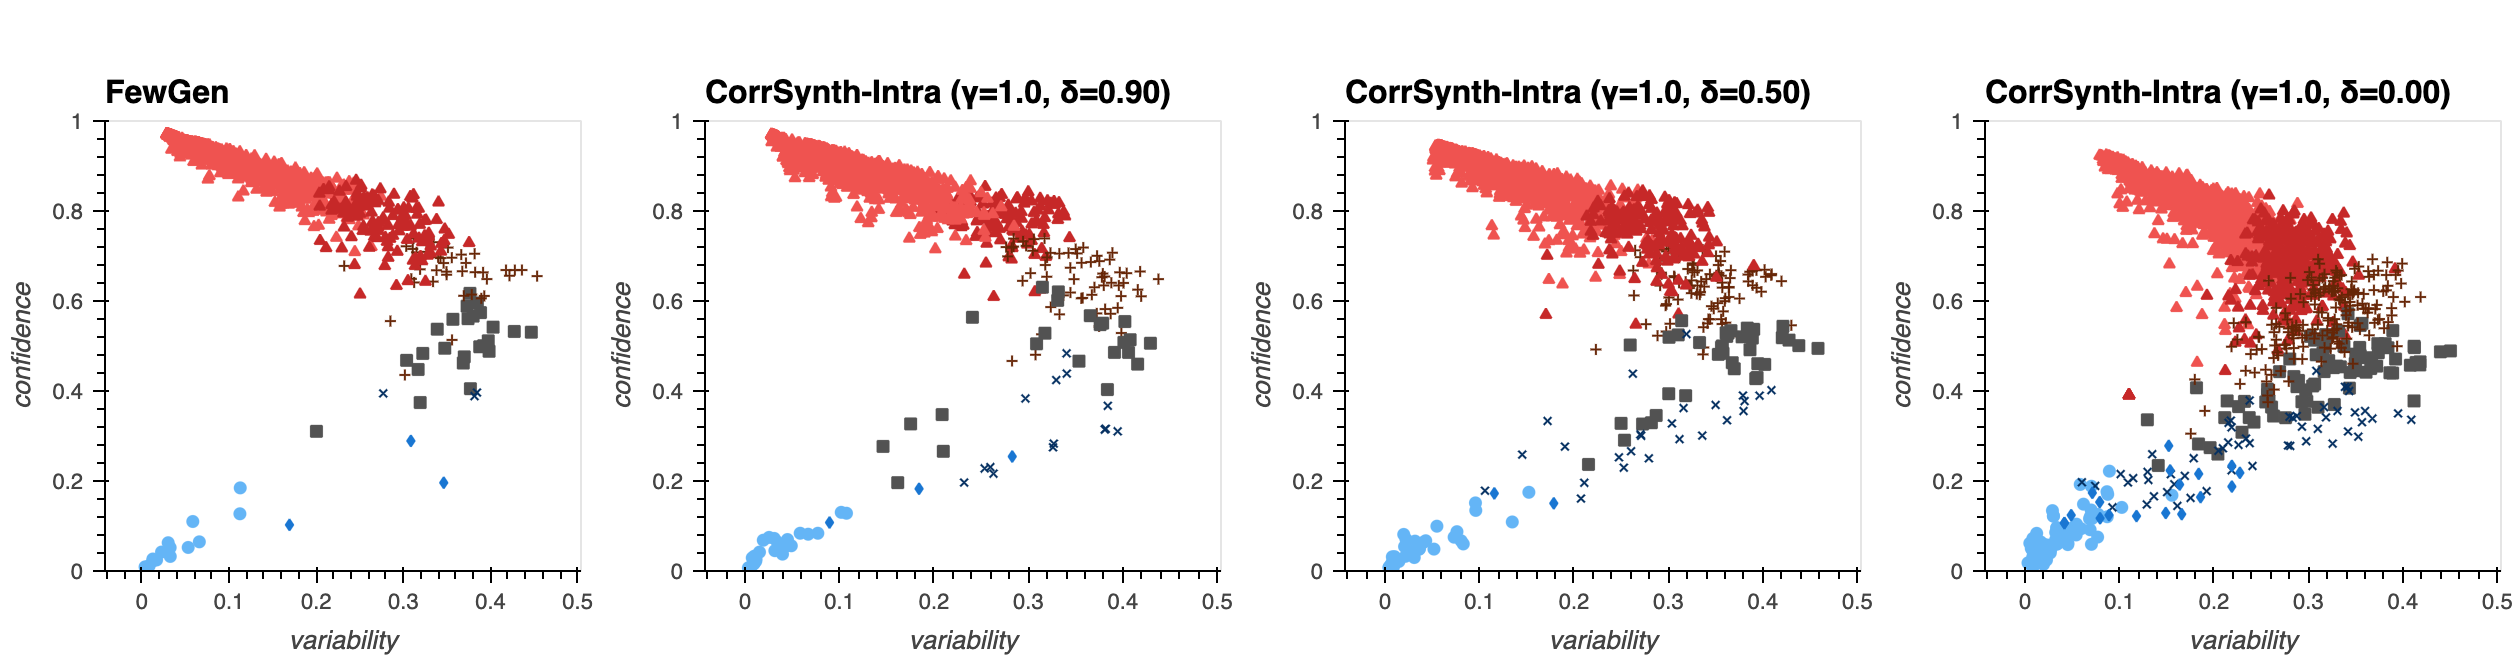
\includegraphics[width=\textwidth]{figure/carto_plots_v2.png}
\vspace{-0.5cm}
\caption{Datamaps for \DistilBERT\ training run on $2$K examples of \ToIHeadlines\ generated using \corrsyn-Intra using Phi-3-mini. \fewgen\ datamap is provided for reference.}
\vspace{-1em}
\label{fig:intra-label-carto}
\end{figure*}

\section{Analysis and Visualizations}
\label{sec:analysis}

\textbf{Effect of Intra-label and Cross-label contrasts:} Given the promising results of our method \corrsyn, we wanted to analyse and visualize the effect of varying Intra-label and cross-label contrasts upon the generations. For this, we obtain the average label-wise cosine similarities of the generations and plot them as heatmaps (see \autoref{fig:cosine}). We specifically study the behavior of our approach in multi-label setting upon \ToIHeadlines\ dataset to emphasize our results. In practice, we use the \texttt{all-mpnet-base-v2} model from SentenceTransformers library to obtain the text representations of each generation. Next, for generations each label $i$ and $j$ in the labelspace, we compute the pairwise cosine similarities of all generations corresponding to label $i$, to that of label $j$. The pairwise cosine similarities are then added and the mean label-wise similarity is computed. We hypothesize that in our approach (Hybrid \corrsyn), if the Intra label contrast is increased, then, within each class the generations should get further away so that the net cosine similarity within the class should reduce across all classes. As we can see in \autoref{fig:cosine_intra}, the diagonals become lighter as we go left to right. On the other hand, if the cross-label contrast is increased net separability between every pair of classes should increase. As expected, we can see in \autoref{fig:cosine_cross}, in the heatmaps the off-diagonal label similarities are becoming lighter as cross contrast is increased. 





\textbf{Effect of $\delta$:} To visualize the effect of varying $\delta$ on the generations obtained through \corrsyn, we plot 2-dimensional representations of the generations. We use Uniform Manifold Approximation and Projection (UMAP)~\cite{mcinnes2020umap} for Dimension Reduction\footnote{https://umap-learn.readthedocs.io/en/latest/} of text representations obtained using \texttt{all-mpnet-base-v2} model. As earlier, we perform this analysis in a multi-label setting with \ToIHeadlines. 

In \autoref{fig:intra_label_umaps}, we can see that as $\delta$ is reduced from $(0.9, 0.5, 0)$, the representations become more and more diffused with each other, leading to overlaps, making the student model hard to learn the decision boundary. For $\delta=0.9$, we can visualize the clusters containing data points from different labels are well-separated, which resonates with our best performing results as well. Note that overlapping/diffused datapoints could be indicators of mislabelled generations as well as hard negatives. 

We hypothesize that as we decrease delta from $0.9$, first we see an increase in hard negative generations than mislabeled generations, whereas after some threshold, the extent of mislabeled generations increase. Thus there is a sweet spot which provides good amount of hard examples with minimal number of wrong generations. We can see this effect in the corresponding cartography plots \cite{swayamdipta-etal-2020-dataset} in \autoref{fig:intra-label-carto} where as we go from left to right, the density of gray and blue points increase but blue points density increases more for much smaller delta than for gray points. The gray points here typically denote hard to learn examples, where as the blue one predominantly represent mislabeled example. These hard negative generations benefit the student model training. %We can see in the corresponding cartography plots in \autoref{fig:intra-label-carto}, we are able to generate more datapoints having low classification confidence and high variability, which in turn benefits the model during training.